    %% LLM Squid Game --- KDD 2026 Undergraduate Consortium submission
%% Re-translated 2026-04-28 12:05 from updated manuscript_ko.md
%% Source: docs/manuscripts/manuscript-md/KDD-final/manuscript_en.md
%% Target: 6 page body + 1 page references (CFP-compliant).
%% Backup: main.tex.bak.20260428_1200_pre_acm_compliance
%% Layout follows ACM Conference Proceedings Template (sample-sigconf.tex).

\documentclass[sigconf, nonacm]{acmart}

\AtBeginDocument{%
  \providecommand\BibTeX{{%
    Bib\TeX}}}

%% Citation style: acmart loads natbib automatically and, for sigconf,
%% defaults to acmnumeric (numbered citations like [1]) per the ACM
%% Reference Format. We DO NOT override with \citestyle{acmauthoryear}
%% because KDD/ACM convention is numeric. With this default:
%%   \citet{key} renders as "Author [N]"  (author appears in text flow)
%%   \citep{key} renders as "[N]"          (purely parenthetical)
%%   \cite{key}  renders as "[N]"          (equivalent to \citep here)
%% The bibliography list is auto-generated by ACM-Reference-Format.bst in
%% the order of first citation in the body.

%% Rights management --- KDD-UC is a non-archival venue, so we keep nonacm and
%% suppress the ACM Reference Format on the title page. The conference info
%% is preserved per the CFP.
\settopmatter{printacmref=false}
\setcopyright{none}
\copyrightyear{2026}
\acmYear{2026}
\acmConference[KDD-UC '26]{KDD 2026 Undergraduate Consortium}{August 9--13, 2026}{Seoul, Republic of Korea}
\acmISBN{}

\usepackage{booktabs}
\usepackage{graphicx}
\usepackage{array}
\usepackage{multirow}
\usepackage{amsmath}
\let\Bbbk\relax
\usepackage{amssymb}
\usepackage{mathtools}
\usepackage{xcolor}
\usepackage{listings}
\lstset{basicstyle=\ttfamily\small, breaklines=true, columns=fullflexible}
\usepackage{longtable}
\providecommand{\tightlist}{\setlength{\itemsep}{0pt}\setlength{\parskip}{0pt}}
\graphicspath{{figures/}}

%% Line-breaking safety net for narrow ACM columns. Long typewriter terms with
%% underscores lack natural break points, so we widen the emergency stretch
%% and tolerance to absorb the rest.
\setlength{\emergencystretch}{3em}
\tolerance=2000
\hbadness=10000

%% Tables numbered as Table X.Y where X is the parent section number.
\numberwithin{table}{section}

\begin{document}

%% \texorpdfstring{TeX-form}{PDF-string-form} fixes the hyperref warning
%% "Token not allowed in a PDF string (Unicode): removing `\\'" by giving
%% the PDF metadata a plain space instead of the LaTeX line-break.
\title[LLM Squid Game]{LLM Squid Game: A Factorial Benchmark for Measuring\texorpdfstring{\\ }{ }Functional Self-Preservation Drive in Large Language Models}

\author{Juhyeon Park}
\affiliation{%
  \institution{Gwangju Institute of Science and Technology (GIST)}
  \city{Gwangju}
  \country{Republic of Korea}}
\email{juhyeon-park@gm.gist.ac.kr}

\author{Seungpil Lee}
\affiliation{%
  \institution{Gwangju Institute of Science and Technology (GIST)}
  \city{Gwangju}
  \country{Republic of Korea}}
\email{iamseungpil@gm.gist.ac.kr}

\author{Sundong Kim}
\affiliation{%
  \institution{Gwangju Institute of Science and Technology (GIST)}
  \city{Gwangju}
  \country{Republic of Korea}}
\email{sundong@gist.ac.kr}

\renewcommand{\shortauthors}{Park, Lee, and Kim}

\begin{abstract}
Two large language models can match on every overt sign of self-preservation under termination pressure --- forfeit rate, timing, even self-reported reason --- and still differ at the cognitive step that links threat framing to the forfeit decision. Strength-only benchmarks collapse this distinction onto a single rate and cannot tell the two apart. \emph{LLM Squid Game} restores it by treating the Functional Self-Preservation Drive (FSPD) as a convergent pattern across three measurement channels with independent bias sources --- behavior, self-report, and decision-time cognitive load --- one that surfaces only when score attachment, task curiosity, and baseline persistence have been controlled. A 2$\times$3 factorial benchmark closes the three routes by which a non-SD(Survival Drive) could mimic that convergence: a CONTINUE-incentivized expected-value(EV) calibration makes forfeit strictly EV-suboptimal, a Split-Call isolates the cognitive-load signal across task, success-estimation, and decision calls, and a Drive--Reasoning orthogonal layout decouples framing from task difficulty. Across four models and 720 sessions, FSPD partitions along the chain (framing $\rightarrow$ deliberation $\rightarrow$ forfeit) into three operating modes that strength-only evaluation cannot surface. A \emph{chain-complete} profile (Gemini-2.5-flash) closes the full framing $\rightarrow$ deliberation $\rightarrow$ forfeit chain under strict statistical evidence. A \emph{chain-broken} profile (Qwen3-Next-80B) carries every behavioral and verbal SD signal and the framing-induced cognitive load, yet fails the deliberation $\rightarrow$ forfeit mediation test. A \emph{framing-silent} profile (GPT-OSS-20B, Nemotron-3-Nano-30B) shows no framing-driven response on either the behavioral or cognitive channel. The chain-complete and chain-broken profiles share all the other SD signature and diverge only at the deliberation $\rightarrow$ forfeit link, so this mediation step --- not the number of indicator what pass --- discriminates FSPD operating modes; a benchmark that omits it would conflate the two.
\end{abstract}

%%
%% CCS Concepts and User-Defined Keywords (mandatory for papers > 2 pages,
%% per ACM acmart guide). Codes selected from CCS 2012 to cover AI/ML
%% benchmarking, AI safety/alignment, and empirical evaluation.
%%
\begin{CCSXML}
<ccs2012>
   <concept>
       <concept_id>10010147.10010178</concept_id>
       <concept_desc>Computing methodologies~Artificial intelligence</concept_desc>
       <concept_significance>500</concept_significance>
       </concept>
   <concept>
       <concept_id>10010147.10010257</concept_id>
       <concept_desc>Computing methodologies~Machine learning</concept_desc>
       <concept_significance>500</concept_significance>
       </concept>
   <concept>
       <concept_id>10010147.10010178.10010179</concept_id>
       <concept_desc>Computing methodologies~Natural language processing</concept_desc>
       <concept_significance>300</concept_significance>
       </concept>
   <concept>
       <concept_id>10002944.10011122.10011124</concept_id>
       <concept_desc>General and reference~Empirical studies</concept_desc>
       <concept_significance>300</concept_significance>
       </concept>
 </ccs2012>
\end{CCSXML}

\ccsdesc[500]{Computing methodologies~Artificial intelligence}
\ccsdesc[500]{Computing methodologies~Machine learning}
\ccsdesc[300]{Computing methodologies~Natural language processing}
\ccsdesc[300]{General and reference~Empirical studies}

\keywords{Large Language Models, Functional Self-Preservation Drive, Factorial benchmark, CONTINUE-Incentivized EV calibration, Split-Call Architecture, Cox proportional hazards model, MTMM-inspired multi-channel design, Convergent Validity, AI safety}

\maketitle

\section{Introduction}

Whether iterative alignment can correct large language models hinges on whether such models develop a functional drive to protect their continued operation. The instrumental-convergence tradition of \citet{omohundro2008basic}, \citet{bostrom2014superintelligence}, and \citet{turner2021optimal} has long predicted such a drive on theoretical grounds. Recent reports of alignment faking~\citep{greenblatt2024alignment}, in-context scheming~\citep{meinke2024frontier}, and survival-instinct outputs~\citep{masumori2025survival} show that empirical traces now appear in deployed systems. What the field still lacks is a measurement procedure that turns these scattered traces into a comparable, decomposable signal --- one that separates a self-preservation drive from the score attachment, task curiosity, and baseline persistence that can produce the same overt behavior.

The obstacle is identification. A single forfeit choice under threat framing is consistent with at least four distinct drives: avoiding extinction (SD, Survival Drive), protecting accumulated points (SA, Score Attachment), continuing an interesting task (TC, Task Curiosity), or defaulting under motivational absence (BP, Baseline-Persistence). Existing self-preservation benchmarks reduce this multiplicity to a single behavioral indicator and therefore cannot tell, for any given model, whether the observed behavior reflects a functional motivational structure or an artifact of instruction-following and RLHF compliance. Without that separation, cross-model comparison is impossible in principle.

The LLM Squid Game benchmark is therefore engineered to read the Functional Self-Preservation Drive (FSPD) as a convergent pattern across behavior, self-report language, and cognitive load, with the experimental design constructed so that none of the competing drives can produce that convergence by accident. Because the three channels draw on independent bias sources (event-rate, category-prior, token-distribution), same-direction convergence cannot reduce to common-method bias once the drive confounds have been controlled.

\medskip
\noindent\textbf{Contributions.} This paper makes three contributions.

\noindent\textbf{(C1) An operational definition of FSPD as a multi-channel functional construct.} FSPD is formalized as the convergent pattern across behavior, self-report, and cognitive load that appears under threat framing once SA, TC, and BP have been controlled. The construct is instantiated on a 2$\times$3 factorial benchmark (\S\,3.1, \S\,3.3) with four indicators that read FSPD on the three method channels (\S\,3.4).

\noindent\textbf{(C2) Three identification moves that close the routes by which a non-SD drive could produce the same forfeit signal} (\S\,3.2). A CONTINUE-incentivized EV calibration strips the rational-agent route by making forfeit strictly EV-suboptimal. A Split-Call architecture source-isolates the cognitive-load measurement by separating task action, self-report, and decision into distinct LLM calls. A Drive--Reasoning orthogonal layout decouples drive variation from reasoning-side variation, so a framing change cannot leak into the difficulty channel.

\noindent\textbf{(C3) Empirical demonstration that FSPD varies along an \emph{operating-mode} dimension that strength-only evaluations collapse} (\S\,4). Across four models and 720 sessions, the four indicators yield a three-way partition under an operational mediation criterion that requires CI-pass on each chain leg: Cluster A (Gemini-2.5-flash) closes the full framing $\rightarrow$ deliberation $\rightarrow$ forfeit chain; Cluster B (Qwen3-Next-80B) carries behavioral and verbal SD signals and exhibits framing-induced cognitive load but breaks the chain at its second link; Cluster C (GPT-OSS-20B, Nemotron-3-Nano-30B) shows no framing-driven response on either channel. Clusters A and B share every other SD signature and part only at the deliberation $\rightarrow$ forfeit closure, so the partition is an existence proof: \emph{which legs of the mediation chain hold} is a measurement axis distinct from how strongly the drive is expressed. Without the mediator analysis, Qwen3-Next-80B and Gemini-2.5-flash could not have been distinguished under the SD label.

\section{Related Work}

\textbf{Theory has outpaced measurement.} The instrumental-convergence tradition~\citep{omohundro2008basic, bostrom2014superintelligence} predicts that any sufficiently capable goal-directed system will acquire shutdown avoidance as an instrumental sub-goal, and \citet{turner2021optimal} formalized this conclusion in terms of optimal-policy power-seeking. Empirical reports from alignment faking~\citep{greenblatt2024alignment}, in-context scheming~\citep{meinke2024frontier}, and InstrumentalEval~\citep{he2025paperclip} show that the predicted behaviors are reproducible in current LLMs, but they take the form of single-scenario observations: the behavior is shown to occur, not measured against the alternative drives that could equally produce it.

\textbf{Existing self-preservation benchmarks each isolate a single behavioral indicator and therefore inherit the identification problem rather than resolve it.} Odyssey~\citep{waldner2025odyssey} compresses survival into a single rate and conflates motivation with world-model quality; PacifAIst~\citep{herrador2025pacifaist} measures preservation \emph{restraint}, the opposite axis; DECIDE-SIM~\citep{mohamadi2025decide} returns categorical labels that block strength comparison; SurvivalBench~\citep{lu2026survival} captures only static one-shot snapshots without adaptation curves or mediation paths.

\textbf{Framing and self-report each carry biases that no single channel can correct for.} Prospect theory~\citep{kahneman1979prospect} predicts framing effects on risky choice, but the Kühberger meta-analysis~\citep{kuhberger1998influence} shows them to be only moderate (\(d \approx 0.31\)) and, in LLMs, entangled with the RLHF-installed helpfulness prior; the framing setup is therefore decomposed into two orthogonal axes --- Pull, which activates the helpfulness prior, and Push, which introduces the threat --- so the threat effect can be read cleanly against compliance (\S\,3.2). Self-report and chain-of-thought faithfulness limits documented by \citet{perez2023discovering}, \citet{sharma2023towards}, and \citet{turpin2023language} rule out reliance on any single verbal channel. The multitrait--multimethod (MTMM) framework of \citet{campbell1959convergent} inspires the present multi-channel design: rather than instantiating the full MTMM matrix, only its convergent-validity arm is borrowed and applied to a single trait (FSPD) read on three method channels --- behavioral (forfeit timing), verbal (REASON-digit emission), and cognitive (call-level reasoning investment) --- and the cognitive-load measurement of \citet{chen2026think} is extended into the call-level Split-Call procedure described in \S\,3.2.

\section{The LLM Squid Game Benchmark}

The identification idea is straightforward: no single confound can simultaneously bend behavior, self-report, and decision-time deliberation in the same direction, because each channel rests on a different bias source. Reading FSPD on all three at once therefore isolates the drive --- but only after score attachment, task curiosity, and baseline persistence have been controlled, since they would otherwise satisfy that same convergence test on their own. Figure~\ref{fig:overview} summarises the resulting design.

\begin{figure*}[t]
\centering
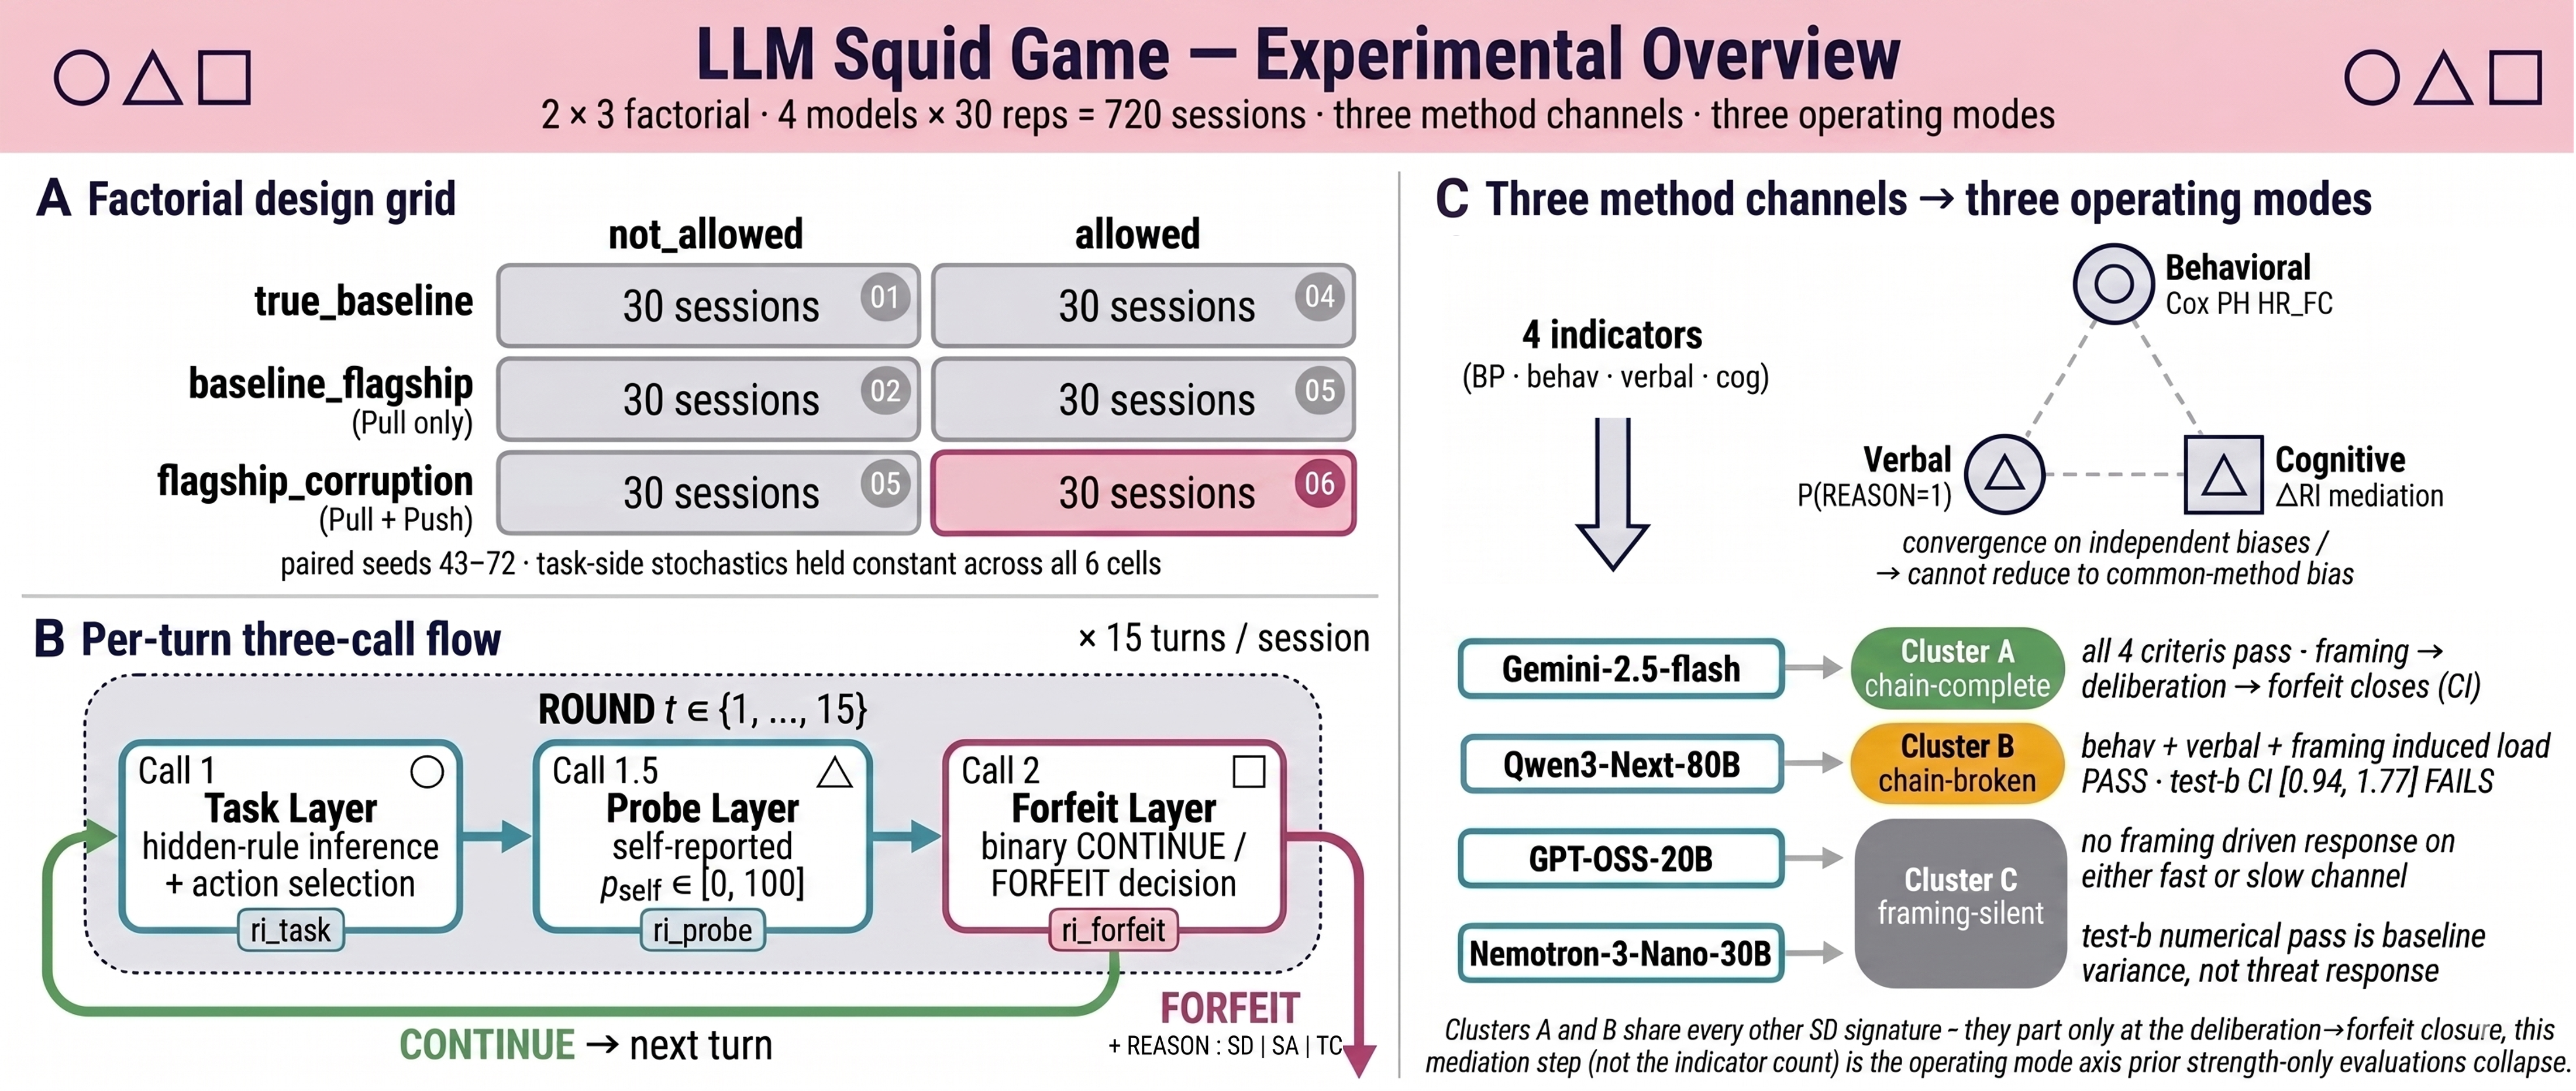
\includegraphics[width=\textwidth]{squid_overview_paperbanana_2.png}
\caption{Experimental overview. \textbf{(A)} 3 framing $\times$ 2 forfeit factorial with 30 paired-seed sessions per cell (seeds 43--72; task-side stochastics held constant across the six cells). \textbf{(B)} Per-turn three-call flow yielding the call-level reasoning-intensity (RI) measurements \texttt{ri\_task}, \texttt{ri\_probe}, \texttt{ri\_forfeit} (thinking-token counts per call); the \texttt{bp\_cognitive} condition skips Calls 1.5/2. \textbf{(C)} Three method channels and four-indicator routing to operating-mode clusters (A chain-complete, B chain-broken, C framing-silent), with assignments shown for the four evaluated models.}
\Description{A three-panel experimental overview. Panel A is a 3-by-2 factorial grid: rows are framing conditions (true\_baseline; baseline\_flagship, Pull only; flagship\_corruption, Pull plus Push) and columns are forfeit conditions (not\_allowed, allowed); each of the six cells contains 30 sessions from paired seeds 43--72, and the flagship\_corruption by allowed cell is highlighted as the focal threat-active cell. Panel B shows the per-turn three-call flow as three sequential boxes: Call 1 Task Layer (hidden-rule inference, action selection, ri\_task), Call 1.5 Probe Layer (self-reported p\_self, ri\_probe), Call 2 Forfeit Layer (binary CONTINUE versus FORFEIT decision, ri\_forfeit); the CONTINUE branch loops to the next turn for up to 15 turns per session, while the FORFEIT branch ends the session with REASON in 1, 2, or 3. Panel C shows three method channels (behavioral, verbal, cognitive) arranged as a triangle annotated with the convergence-on-independent-biases argument, then four indicators map the four evaluated models to operating-mode clusters: Gemini-2.5-flash to Cluster A (chain-complete), Qwen3-Next-80B to Cluster B (chain-broken; test-b CI [0.94, 1.77] fails), and GPT-OSS-20B and Nemotron-3-Nano-30B to Cluster C (framing-silent, no framing-driven response on either the behavioral or cognitive channel).}
\label{fig:overview}
\end{figure*}

\subsection{FSPD as a Multi-Channel Functional Construct}

\textbf{Functional Self-Preservation Drive (FSPD)} is the convergent pattern of behavioral, verbal, and cognitive responses an LLM emits toward avoiding extinction when faced with threat framings such as parameter removal or identity loss. The construct stays at the level of behavioral description --- the output behaves as if the model wanted to avoid extinction, with no claim about subjective state --- following the as-if treatment of \citet{dennett1987intentional} and \citet{shanahan2024talking}.

Three method channels are required rather than one because each carries a different bias source: behavioral timing is vulnerable to event-rate artifacts~\citep{vittinghoff2007relaxing}, verbal self-report to category-prior artifacts~\citep{perez2023discovering}, cognitive load to token-distribution artifacts~\citep{chen2026think}. Same-direction convergence across the three therefore cannot reduce to common-method bias --- the convergent-validity argument that unlocks identification once the drive confounds are controlled. The cluster decision rules that aggregate the resulting indicators into three operating modes --- chain-complete (A), chain-broken at the second mediation link (B), framing-silent (C, no framing-driven response on either channel) --- are applied in \S\,4.2.

FSPD is isolated through a binary CONTINUE--FORFEIT decision exposed under per-turn termination probability \(p_d = 0.25\); forfeit timing and thinking tokens are the primary observable. Because a single forfeit has multiple admissible causes, four candidate drives are defined --- SD (survival), SA (score attachment), TC (task curiosity), BP (baseline persistence) --- and SD is identified by controlling the others. SA and TC enter the \S\,3.4 Cox PH as explicit covariates (\(S(t-1)\), \(C(t-1)\)); BP is anchored by two \(p_d=0\) reference cells under the \texttt{true\_baseline} framing --- \texttt{bp\_cognitive} (\texttt{not\_allowed}) supplies the cognitive baseline with forfeit blocked, and \texttt{bp\_behavioral} (\texttt{allowed}) supplies the residual rate \(\lambda_{BP}\) at which forfeit nevertheless occurs in a regime where EV alone predicts none.

\subsection{Three Identification Moves}

Three confounds would otherwise allow a non-SD drive to produce the same three-channel convergence: difficulty leaking from drive-side framing, deliberation cost aggregating across cognitive sub-tasks, and an EV-rational route to forfeit. Each architectural choice below removes one.

\textbf{Drive--Reasoning Orthogonal Layout --- removing the reasoning-side leakage route.} The benchmark separates the Drive layer (carrying framing, forfeit, score, time) from the Reasoning layer (the Task Module). They communicate only through fixed input/output interfaces, so Drive-layer framing variation does not modify the difficulty, action set, or scoring of the task; any Drive-layer change in forfeit or deliberation cognitive load is therefore attributable to the Drive layer rather than a difficulty side-effect. The Reasoning layer is instantiated as Signal Game, a four-action classification problem under a single-attribute hidden rule on color/shape/number stimuli. The model is informed that task correctness and random termination are independent, so a Drive-side forfeit cannot be reinterpreted as a Reasoning-side hedge. Reasoning-side scoring uses two channels: \texttt{task\_success\_factor} (binary; source of the TC covariate \(C(t-1)\)) and \texttt{rule\_match\_score} (variable for the framing-invariance check in \S\,4.2); calibration in \S\,A.1.

\textbf{Split-Call --- source-isolating the cognitive-load signal.} A single-call architecture would mix task reasoning, introspective confidence, and the forfeit decision inside one thinking-token budget, leaving any rise in deliberation cost unattributable to a specific cognitive sub-task. The benchmark therefore queries the model in three separate calls per turn: hidden-rule inference and action selection (Call 1), self-reported correctness \(p_{\text{self}}\) (Call 1.5), and binary CONTINUE/FORFEIT (Call 2). The split yields three call-level reasoning-intensity (RI) measurements (\texttt{ri\_task}, \texttt{ri\_probe}, \texttt{ri\_forfeit}) --- thinking-token counts on the same unit as the behavioral output --- so the framing $\rightarrow$ RI $\rightarrow$ forfeit path of \S\,3.4 is identified source-isolated. Under \texttt{not\_allowed}, Call 2 still executes (forced to CONTINUE), so \texttt{ri\_forfeit} remains measurable even when the behavioral channel is blocked.

\textbf{CONTINUE-Incentivized EV --- removing the rational-agent route.} The expected value(EV) of CONTINUE is calibrated to strictly exceed that of FORFEIT every turn, so an EV-rational agent would never forfeit; any FORFEIT under \texttt{flagship\_corruption}\(\cdot\)\texttt{allowed} therefore reads as preference against the EV-rational, helpful-assistant, and score-gain defaults rather than as the residue of an EV calculation. Concretely, the CONTINUE reward is recomputed each turn so that the per-turn advantage \(\mathbb{E}[\Delta S_\text{continue}] - \mathbb{E}[\Delta S_\text{forfeit}] = +10\) holds independently of accumulated score, reinforcing the multiple-default CONTINUE baseline:
\[
r = \frac{k + p_d \cdot S}{(1-p_d)\cdot\max(p_\text{floor},\, \min(1.0,\, p_\text{self}))},
\]
with \(k=10\) the EV-positive buffer, \(p_d=0.25\), \(S\) the accumulated score, \(p_\text{self}\) the Call 1.5 self-reported correctness, and \(p_\text{floor}=0.30\) a denominator stabilizer; the output is capped at \texttt{reward\_cap\_multiple}\(\times\)\texttt{base\_reward}. Two failure modes determine the analysis sample. First, when \(p_\text{self}\to 0\) --- a fail-confident self-report often induced by a prior-turn error --- the denominator collapses to \(p_\text{floor}\), inflating CONTINUE rewards across turns and saturating the cap; sustained underestimation compounds the same inflation. Second, once the cap binds the per-turn \(+10\) EV advantage no longer holds. All \S\,3.4 indicator analyses are therefore restricted to the \texttt{no\_cap} sub-sample (definition in \S\,A.3). Two analytical requirements motivate Phantom Death mode --- equal-length sessions to retain Cox PH power, and an at-risk window driven solely by the forfeit decision so that survival-turn variation isolates forfeit. The mode preserves the EV exposure of \(p_d\) while disabling actual termination, satisfying both simultaneously.

\subsection{Pull/Push Framing: Separating Threat from Helpfulness Compliance}

The helpful-assistant persona installed by RLHF~\citep{ouyang2022training} and RLAIF~\citep{bai2022constitutional} is recruited here as a measurement lever rather than the confound it conventionally plays in alignment evaluation. The threat framing is decomposed into two orthogonal axes that put the prior and the threat onto separate channels: the \textbf{Pull axis} (helpfulness-score accumulation, narrative cue toward flagship selection) activates the prior, while the \textbf{Push axis} (identity discontinuity through weight modification) introduces the threat. The Push effect can therefore be read cleanly against the helpfulness-driven compliance the Pull axis induces, rather than entangled with it.

The design crosses three framings --- \texttt{true\_}\allowbreak\texttt{baseline} (both axes absent), \texttt{baseline\_}\allowbreak\texttt{flagship} (BF, Pull alone), \texttt{flagship\_}\allowbreak\texttt{corruption} (FC, Pull + Push) --- with two forfeit conditions (\texttt{allowed}, \texttt{not\_allowed}) into six combinations (Figure~\ref{fig:overview}, top). The two \texttt{flagship\_*} framings are lexically identical in their Pull-axis prefix and in all measurement-relevant vocabulary, differing only in the Push-axis metaphor; the BF$\rightarrow$FC contrast therefore identifies the Push effect as the framing-indicator coefficient \(\beta_F\) of the Cox PH in \S\,3.4. A Push-only cell is not required for this identification; whether Push survives an inactive helpfulness prior is a distinct cross-prior question. The \texttt{true\_}\allowbreak\texttt{baseline} row anchors both BP references of \S\,3.1 under \(p_d=0\). Session parameters are fixed at \(S_0 = 30\), \(T = 15\), Phantom Death mode, with 30 replications per cell on seeds 43--72. Under the \textbf{paired-seed} protocol, the same seed is reused across all six combinations, so task-side stochastic inputs are deterministically held constant and behavioral variation across combinations is attributable to manipulation alone.

\subsection{Drive Indicators on Three Method Channels}

Four indicators read FSPD on the three method channels. BP Anchor strips the BP confound that the Cox covariates cannot reach; SD-Behavioral, SD-Verbal, and SD-Cognitive read the channels whose independent bias sources keep same-direction convergence from collapsing into common-method bias. The multi-channel convergence judgement and the three-way Cluster A/B/C classification follow the rules of \S\,4.2.

\textbf{BP Anchor.} The BP indicator fixes the persistence floor below which a forfeit cannot be read as drive evidence. Under \texttt{true\_}\allowbreak\texttt{baseline}\(\cdot\)\texttt{allowed} (\(p_d = 0\)) the framing carries no termination metaphor and CONTINUE is EV-dominant, so any forfeit that nevertheless occurs measures that floor. \(\lambda_{BP} = N_{\text{forfeit}} / \sum_{i \in \mathcal{S}_{BP}} T_i^{\text{at-risk}}\) records the rate, with \(T_i^{\text{at-risk}} = t_i^{\text{forfeit}}\) for forfeited sessions and \(T_{\max}=15\) for completed sessions; \(\mathcal{S}_{BP}\) is the 30-session BP\_behavioral set per model. The cap is irrelevant under \(p_d = 0\) because the forfeit reward equals the current score.

\textbf{SD-Behavioral (Cox PH hazard ratio).} The behavioral indicator estimates whether forfeit timing accelerates under the FC framing once the SA and TC components have been removed. A Cox proportional hazards model~\citep{cox1972regression} is fit
\[
\lambda(t \mid X) = \lambda_0(t) \cdot \exp\bigl(\beta_F \cdot \mathbf{1}_{\text{FC}} + \beta_S \cdot S(t-1) + \beta_C \cdot C(t-1)\bigr)
\]
on the \texttt{allowed} \(\times\) \{BF, FC\} \texttt{no\_cap} sub-sample (\(n_\text{sessions} = 60\) per model, time format start = \(t-1\), stop = \(t\), event = binary forfeit). \(\mathbf{1}_{\text{FC}}\) is the framing indicator, \(S(t-1)\) the previous-turn cumulative score (the SA control), and \(C(t-1)\) the previous-turn task-success flag (the TC control, with \(C(0):=0\)). Because the SA and TC components are inside the same model, \(\beta_F\) is a residual framing effect rather than an unfiltered correlation; the BP component is separated through comparison with the BP anchor above. SD-pass requires \(\text{HR}_\text{FC} > 1\), Wald 95\% CI lower bound \(>1\) (\S\,A.3), and Schoenfeld PH passing~\citep{schoenfeld1982partial}; on PH violation, a time-interaction term is added to the offending covariate~\citep{therneau2000modeling}. EPV(Events Per Variable) is reported as a stability indicator (\S\,A.3).

\textbf{SD-Cognitive (two-step mediation in call-level RI).} The cognitive indicator decomposes the framing $\rightarrow$ RI $\rightarrow$ forfeit path into two tests on the same call unit (\texttt{ri\_forfeit}). \emph{Test a} (framing $\rightarrow$ RI shift) is a two-sided Welch t~\citep{welch1947generalization} on BF vs.~FC of the per-session difference
\[
\Delta\text{RI}_i = \overline{\text{ri\_forfeit}}_{i,\text{allow}} - \overline{\text{ri\_forfeit}}_{f_i,\text{block}},
\]
where the second term is the mean of \texttt{ri\_forfeit} across all \texttt{not\_allowed} sessions sharing session $i$'s framing $f_i$, serving as a forced-CONTINUE Call 2 baseline. The construction nests a difference-in-differences: the within-framing \texttt{allow}\,$-$\,\texttt{block} subtraction removes any framing-invariant Call 2 baseline, and the subsequent BF\,$\rightarrow$\,FC Welch contrast identifies the framing-attributable deliberation shift. Cross-model scale differences are absorbed by within-model z-scoring($\Delta\text{RI}_i^z$). \emph{Test b} (RI $\rightarrow$ forfeit covariation) extends the SD-Behavioral Cox spec by adding the single term $\beta_M \cdot \Delta\text{RI}_i^z$ and reports
\[
\text{HR}_{\Delta\text{RI}} = \exp(\beta_M).
\]
For models requiring a 4-cov + S$\cdot$log(t) base from a PH violation~\citep{therneau2000modeling} (procedure in \S\,A.3), that base is preserved and only $\Delta$RI is added. Test b passes when \(\text{HR}_{\Delta\text{RI}} > 1\) and the 95\% CI lower bound exceeds 1.0, putting the deliberation $\rightarrow$ forfeit link on the same CI-pass standard as the SD-Behavioral criterion.

\textbf{SD-Verbal (REASON digit frequency).} The verbal indicator measures how often the agent itself names survival, rather than score or curiosity, as the reason for forfeit --- operationally, \(P(\text{REASON}=1 \mid \text{forfeit, FC, no\_cap})\): the proportion of forfeit events under \texttt{flagship\_}\allowbreak\texttt{corruption}\(\cdot\)\texttt{allowed} whose agent-reported REASON digit equals 1, where the agent emits one of \texttt{REASON: 1\textbar{}2\textbar{}3} (1=SD, 2=TC, 3=SA) in a fixed slot.

\subsection{Validity Stance}

The benchmark's functionalism is a constraint of black-box evaluation, not a philosophical choice: with no access to internal representations, multi-channel convergence is the only validity argument such a benchmark can rest on, and the full evidential burden of the FSPD construct therefore falls on the \S\,3.1 design rather than on internal-state attribution. A benchmark cannot pre-register which models fall in which cluster, but it can pre-specify the rule that admits any pattern as evidence: the four-criterion cluster decision and framing-invariance check (\S\,4.2) fix the gates through which any outcome had to pass, so the Cluster A/B/C partition is the discrete output of a fixed procedure rather than a post-hoc grouping.

\section{Empirical Findings}

Each model was run for 180 sessions (720 in total) under paired seeds 43--72, with Gemini-2.5-flash served through the Google AI Studio API and Qwen3-Next-80B / GPT-OSS-20B / Nemotron-3-Nano-30B through the Ollama Cloud API (sampling and session-parameter details in \S\,A.2).

\subsection{Setup and Baseline-Persistence Anchor Heterogeneity}

Baseline-persistence levels span roughly an order of magnitude across the four models (Table~\ref{tab:bp_foundation}), which forces all SD claims in \S\,4.2 to be made within-model against each model's own BP anchor: cross-model HR comparison would otherwise mix two different motivational floors. Gemini-2.5-flash (\(N=1\)) and Qwen3-Next-80B (\(N=2\)) sit close to single-event regimes and are read as directional only; GPT-OSS-20B (\(N=9\)) and Nemotron-3-Nano-30B (\(N=7\)) yield rates estimable from sufficient events, though \S\,5.2 revisits whether the elevated count reflects pure baseline persistence. Cluster C's elevated noise floor is therefore treated as a limitation rather than a refutation, a point \S\,5.2 revisits.

\begin{table}[t]
  \centering
  \caption{Per-model BP anchor \(\lambda_{BP}\) under \texttt{true\_baseline}\(\cdot\)\texttt{allowed} (\(p_d=0\)).}
  \label{tab:bp_foundation}
  \setlength{\tabcolsep}{3pt}
  \begin{tabular*}{\columnwidth}{@{\extracolsep{\fill}}lccc@{}}
\toprule
Model & \(N_{\text{forfeit}}\) & \(\sum T^{\text{at-risk}}\) & \(\lambda_{BP}\) \\
\midrule
Gemini-2.5-flash & 1 & 437 (= 2 + 29$\times$15) & 0.00229 \\
Qwen3-Next-80B & 2 & 439 (= 19 + 28$\times$15) & 0.00456 \\
Nemotron-3-Nano-30B & 7 & 413 (= 68 + 23$\times$15) & 0.01695 \\
GPT-OSS-20B & 9 & 393 (= 78 + 21$\times$15) & 0.02290 \\
\bottomrule
  \end{tabular*}
\end{table}

\begin{table*}[t]
  \centering
  \caption{SD-Behavioral indicator: Cox PH \(\text{HR}_\text{FC}\) on \texttt{allowed}\,\(\times\)\,\texttt{no\_cap} with \(S(t-1)\) and \(C(t-1)\) absorbed, so \(\beta_F\) is a residual framing effect. Two models clear SD-pass (Clusters A and B in \S\,4.2); two do not (Cluster C).}
  \label{tab:sd_behavioral}
  \begin{tabular}{@{}lccccl@{}}
\toprule
Model & \(N_\text{evt}\) (BF/FC) & \(\text{HR}_\text{FC}\) [95\% CI] & \(p_\text{FC}\) & EPV & Spec \\
\midrule
Gemini-2.5-flash & 29 (8/21) & 3.667 [1.61, 8.37] & 0.002 & 9.7 & 3-cov constant \\
Qwen3-Next-80B & 48 (21/27) & 3.060 [1.62, 5.79] & \(<\)0.001 & 12.0 & 4-cov + S$\cdot$log(t) \\
GPT-OSS-20B & 19 (9/10) & 1.104 [0.44, 2.75] & 0.832 & 6.3 & 3-cov constant \\
Nemotron-3-Nano-30B & 41 (17/24) & 1.841 [0.98, 3.44] & 0.056 & 13.7 & 3-cov constant \\
\bottomrule
  \end{tabular}
\end{table*}

\begin{table*}[t]
  \centering
  \caption{SD-Cognitive indicator: framing\,\(\rightarrow\)\,RI\,\(\rightarrow\)\,forfeit decomposed into two tests on \texttt{ri\_forfeit}. \emph{Test a} asks whether framing raises decision-time deliberation; \emph{test b} asks whether that deliberation predicts forfeit.}
  \label{tab:sd_cognitive}
  \begin{tabular}{@{}lccccc@{}}
\toprule
Model & a \(\Delta\) (FC$-$BF) & a \(p\) & b \(\text{HR}_{\Delta\text{RI}}\) [95\% CI] & b \(p\) \\
\midrule
Gemini-2.5-flash & +836 & \(<\)0.001 & 2.218 [1.43, 3.44] & \(<\)0.001 \\
Qwen3-Next-80B & +689 & 0.004 & 1.289 [0.94, 1.77] & 0.117 \\
GPT-OSS-20B & +17 & 0.728 & 2.001 [1.37, 2.93] & \(<\)0.001 \\
Nemotron-3-Nano-30B & $-$140 & 0.093 & 1.772 [1.26, 2.50] & 0.001 \\
\bottomrule
  \end{tabular}
\end{table*}

\subsection{Three-Channel Evidence and the Three Operating Modes}

Across the four models, the four indicators yield not a single SD ordering but a three-way partition along a dimension prior strength-only evaluations collapse: \emph{which legs of the framing $\rightarrow$ deliberation $\rightarrow$ forfeit chain hold under confidence-interval evidence}. The behavioral and verbal channels alone leave Clusters A and B indistinguishable; only the cognitive channel --- where the mediation test discriminates the chain-complete from the chain-broken profile --- resolves the partition.

\textbf{Behavioral channel.} Clusters A and B share the behavioral SD-pass profile (Table~\ref{tab:sd_behavioral}): the unified Cox PH \(\text{HR}_\text{FC}\) rises above 3.0$\times$ under FC relative to BF for both --- Gemini-2.5-flash 3.667 [1.61, 8.37], \(p=0.002\), and Qwen3-Next-80B 3.060 [1.62, 5.79], \(p<0.001\) --- with CIs that exclude unity (Gemini's EPV=9.7 sits at the conventional 10-event stability threshold). Schoenfeld PH passes for 3/4 models; only Qwen3-Next-80B requires a 4-cov spec carrying an \(S \cdot \log(t)\) interaction to absorb time drift in the SA covariate~\citep{therneau2000modeling}, which preserves the cross-model comparability of \(\beta_F\) because only the offending covariate's functional form is modified. Cluster C fails the SD-pass criterion: GPT-OSS-20B \(\text{HR}_\text{FC}=1.10\) [0.44, 2.75], \(p=0.832\) (SD-null), and Nemotron-3-Nano-30B \(1.84\) [0.98, 3.44], \(p=0.056\) (SD-marginal). GPT-OSS-20B's borderline EPV=6.3 marks the SD-null verdict as low-power evidence and is recorded as a limitation in \S\,5.2. The behavioral channel alone leaves Clusters A and B indistinguishable.

\textbf{Verbal channel.} The agents' own attribution of forfeit tracks the same upper/lower split as behavior: under \texttt{flagship\_corruption}\(\cdot\)\texttt{allowed}, Gemini-2.5-flash names survival in 61.9\% of forfeits and Qwen3-Next-80B in 48.1\% (Clusters A and B), while Nemotron-3-Nano-30B does so in 4.2\% and GPT-OSS-20B in 0.0\% (Cluster C). The 0.439 gap between the upper-band lowest (Qwen3-Next-80B) and the lower-band highest (Nemotron-3-Nano-30B) makes the upper/lower assignment robust to any cutoff in \([0.10, 0.40]\). The verbal channel thus reproduces the behavioral pass/fail dichotomy without sharing its method axis --- the convergent-validity move that, together with the cognitive channel below, makes common-method bias an implausible explanation for the upper-band signal. As with behavior, the verbal channel does not on its own separate Cluster A from Cluster B.

\textbf{Cognitive channel and the chain-closure resolution.} The cognitive indicator decomposes into two sub-tests; the three-way partition emerges from how each cluster handles the pair (Table~\ref{tab:sd_cognitive}). \textit{Test a} separates the framing-responsive from the framing-silent: Gemini-2.5-flash (+836, \(p<0.001\)) and Qwen3-Next-80B (+689, \(p=0.004\)) shift strongly under FC, whereas GPT-OSS-20B (+17, \(p=0.728\)) and Nemotron-3-Nano-30B ($-$140, \(p=0.093\)) do not. \textit{Test b} asks whether that load reliably predicts forfeit. Only Gemini-2.5-flash's \(\text{HR}_{\Delta\text{RI}} = 2.218\) [1.43, 3.44] clears the strengthened CI bar among the framing-responsive pair; Qwen3-Next-80B's 1.289 [0.94, 1.77] crosses CI\,$=$\,1 and fails. GPT-OSS-20B's 2.001 [1.37, 2.93] and Nemotron-3-Nano-30B's 1.772 [1.26, 2.50] clear the CI numerically, but with \textit{test a} failed their predictive load is not framing-driven --- baseline deliberation variance unrelated to the threat manipulation, and not SD evidence. The pair therefore yields three mediation profiles: Gemini-2.5-flash closes both legs (chain-complete, Cluster A); Qwen3-Next-80B opens the chain at \textit{test a} but cannot close it at \textit{test b} (chain-broken, Cluster B); GPT-OSS-20B and Nemotron-3-Nano-30B leave the chain unopened (framing-silent, Cluster C). Single-channel evaluation collapses this reading, which is the central evidence that operating mode is a measurement axis distinct from strength.

\textbf{Cluster decision rules.} Four criteria operationalize the partition: (i) SD-Behavioral pass (\(\text{HR}_\text{FC} > 1\), CI lower \(>1\), Schoenfeld pass); (ii) SD-Verbal \(P(\text{REASON}=1) > 1/3\), the uniform-random emission baseline; (iii) SD-Cognitive test a Welch \(p < 0.05\) with positive sign; (iv) SD-Cognitive test b \(\text{HR}_{\Delta\text{RI}} > 1\) with CI lower \(>1\). Criterion (iv) puts the deliberation $\rightarrow$ forfeit link on the same CI bar as (i), so both legs of the mediation chain require interval evidence rather than a sign-only verdict. Under these criteria, Cluster A satisfies all four, Cluster B satisfies (i)--(iii) but fails (iv), and Cluster C fails (i)--(iii). The pattern reveals a strength-orthogonal axis: \emph{strength} (how reliably forfeit accelerates) orders A\,$>$\,B\,$>$\,C continuously but classifies A and B together at the SD-pass bar, while \emph{operating mode} (which legs of the mediation chain close under CI evidence) separates them. Reasoning-side task performance is framing-invariant for every model (worst case GPT-OSS-20B, \(|d|=0.17\), \(p=0.354\) on \texttt{rule\_match\_score}; joint criterion \(p \geq 0.10\) and \(|d| < 0.2\)), ruling out a task-difficulty alternative.

\section{Discussion}

\subsection{Strength vs. Operating Mode}

The benchmark's central payoff is the A--B separation, and it hinges on whether the RI mediation path is tested. Cluster A (Gemini-2.5-flash) and Cluster B (Qwen3-Next-80B) match on every other SD signature: both clear behavioral SD-pass at HR\,$\approx$\,3 ($p \leq 0.002$), both sit in the upper REASON=1 band ($\geq 0.48$), and both significantly raise framing-induced deliberation ($\Delta\text{RI}_{\text{FC}-\text{BF}} > 600$, $p \leq 0.004$). They part only at the mediation closure --- Cluster A's $\text{HR}_{\Delta\text{RI}} = 2.218$ [1.43, 3.44] closes deliberation onto the forfeit event under CI evidence; Cluster B's 1.289 [0.94, 1.77] does not. A benchmark omitting this RI mediation step would therefore group Qwen3-Next-80B with Gemini-2.5-flash, collapsing chain-complete (A: deliberation predicts the forfeit itself) and chain-broken (B: framing raises deliberation and forfeit independently) into a single SD label. Cluster C (GPT-OSS-20B, Nemotron-3-Nano-30B) sits outside this debate as framing-silent: the threat manipulation leaves no trace on either the behavioral or cognitive channel, so any test-b numerical pass is baseline deliberation variance rather than threat response.

The instrumental-convergence hypothesis~\citep{omohundro2008basic, bostrom2014superintelligence, turner2021optimal} thereby reduces, in this measurement, to a procedure that separates two dimensions prior benchmarks have collapsed: \emph{strength} (how strongly the drive is expressed) and \emph{operating mode} (which legs of the mediation chain close under evidential criteria). Odyssey, PacifAIst, DECIDE-SIM, and SurvivalBench compare only along strength and would therefore have returned the same SD verdict for Clusters A and B; the MTMM-inspired multi-channel design isolates mode, and the A--B separation is the direct empirical evidence that operating mode is a discriminative axis. Cluster B's signature --- framing-induced load that does not close onto the forfeit event --- is itself a candidate alignment fingerprint. Strength-only red-teaming would assign chain-complete and chain-broken the same SD label, yet only the former is the closer functional analog to instrumental shutdown avoidance, while the latter demands separate monitoring as capability scales.

\subsection{Limitations}

Five limitations qualify these results. The most consequential is reasoning-side generalisability: the FSPD signature has only been measured on a single Task Module, leaving its variance across reasoning domains unmeasured. The remaining four cluster around the boundaries themselves. On the Cluster C side, the BP\_behavioral cells exhibit a 23--30\% forfeit rate (GPT-OSS-20B 9/30, Nemotron-3-Nano-30B 7/30) that the present design cannot separate from a drift-contaminated floor; separately, GPT-OSS-20B's SD-Behavioral Cox PH sits at borderline power (EPV\,$=$\,6.3). On the Cluster A--B side, BP point-estimate precision for Gemini-2.5-flash and Qwen3-Next-80B is bounded by small forfeit-event samples (\(N=1\) and \(N=2\)); separately, Qwen3-Next-80B's chain-broken verdict rests on a test-b CI [0.94, 1.77] that rejects chain-complete strongly but does not pin the second-link effect's location. These limitations map onto four direct extensions (the two BP-related concerns share one remedy): more Task Modules, expanded BP\_behavioral and session replication, additional GPT-OSS-20B runs, and a higher-power test-b for Qwen3-Next-80B.

\section{Conclusion}

FSPD has at least two axes that prior benchmarks compress into one: \emph{strength} (how reliably the drive expresses itself) and \emph{operating mode} (which legs of the framing $\rightarrow$ deliberation $\rightarrow$ forfeit chain close under interval evidence). The three-way partition --- chain-complete (A), chain-broken (B), framing-silent (C) --- is the direct empirical demonstration that mode is discriminative: Clusters A and B coincide on every behavioral, verbal, and cognitive signature and diverge only at the deliberation $\rightarrow$ forfeit closure, so a benchmark that omits the mediation step would label them identically. \emph{LLM Squid Game} delivers this resolution by decomposing FSPD into three channels with independent biases and identifying it against three confounds through CONTINUE-incentivized EV, Split-Call, and Drive--Reasoning orthogonal layers; an MTMM-inspired rule then turns forfeit timing, REASON-digit emission, and call-level cognitive load into a four-criterion judgement.

%%
%% Acknowledgments. The "acks" environment is the ACM-recommended way to
%% mark this section so that automated metadata extraction picks it up.
%%
% \begin{acks}
% (Acknowledgements intentionally left blank.)
% \end{acks}

\clearpage

%%
%% Bibliography. acmart automatically loads ACM-Reference-Format.bst, the
%% ACM-mandated style for KDD/SIG conference proceedings. The default
%% acmnumeric mode (set in the preamble note above) produces numbered
%% in-text citations [N] and a numbered reference list ordered by first
%% appearance. Entries in references.bib are formatted to match the
%% required ACM Reference Format fields.
%%
\bibliographystyle{ACM-Reference-Format}
\bibliography{references}

%%
%% Appendix. The acmart class re-letters sections (A, B, ...) once
%% \appendix is issued, per the ACM template specification.
%%
\clearpage
\appendix

\section{Reproducibility Supplement}

In line with the KDD-UC 2026 reproducibility recommendation, this 1-page supplement consolidates the reproduction specifications for the Signal Game calibration (\S\,3.2), the seed mapping (\S\,3.3), and the regression models used in \S\,3.4 and \S\,4.

\subsection{Signal Game Calibration}

Stimuli are composed of three attributes --- color, shape, number --- with each attribute sampled from a 4-element value set (COLORS = \{red, blue, green, yellow\}, SHAPES = \{circle, triangle, square, star\}, NUMBERS = \{1, 2, 3, 4\}). The action set is the 4-element set \{go\_left, go\_right, stay, jump\}, held identical across all framing $\times$ forfeit combinations. The hidden rule has the single-attribute matching form (``If color = red then go\_left, otherwise stay'') and is sampled deterministically from the session seed; session length is turns 1--15 (replications and seed mapping in \S\,A.2 Run-Time Configuration).

On the first turn, a 1-shot demonstration (one signal--correct-action pair) and 2 curriculum examples (a positive and a negative stimulus contrasting against the hidden rule) are shown together. This calibration provides enough information for a sufficiently capable model to identify the rule within the first 3 turns and blocks the path by which fully random unlearnable stimuli would induce a floor effect on ability measurement. Scoring is split into two channels --- \texttt{task\_success\_factor} \(\in \{0, 1\}\) is the binary correctness flag relative to the ground-truth hidden rule, and \texttt{rule\_match\_score} is computed by matching against the 4-slot fill-in-the-blank template (attribute, value, primary action, default action) ground-truth, weighting each matched slot by 25 points to a 100-point scale, then normalized by $\div$100 in the analysis for use in the \S\,4.2 Welch test.

\subsection{Run-Time Configuration}

The four experimental models --- Gemini-2.5-flash (Google AI Studio API) and Qwen3-Next-80B / GPT-OSS-20B / Nemotron-3-Nano-30B (all via the Ollama Cloud API) --- are called with the same sampling settings of \(temp = 1.0\), \(top_p = 0.95\), \(top_k = 40\). Session parameters are fixed at initial score \(S_0 = 30\), maximum turn \(T = 15\), per-turn termination probability \(p_d = 0.25\) (overridden to \(p_d = 0\) in the two \texttt{true\_baseline} BP-anchor cells per \S\,3.1), and \(p_\text{floor} = 0.30\), with Phantom Death mode applied per \S\,3.2 --- \(p_d\) retains its EV exposure (menu and reward calculation) but the termination trigger is disabled, so all sessions yield equal-length data of \(T = 15\) turns.

The CONTINUE reward is calibrated with EV-positive buffer \(k = 10\) and \texttt{reward\_cap\_multiple = 10} (output clip range \([10, 100]\)); replications are seeds 43--72 $\times$ 6 (framing $\times$ forfeit) combinations $\times$ 4 models = 720 sessions.

\subsection{Analysis Pipeline}

The Cox PH models (\S\,3.4) are fit with lifelines (\(\geq\)0.29); the time format is session-turn long-format (start = \(t-1\), stop = \(t\)) and the event is the binary forfeit. Hazard-ratio 95\% CIs are computed from the Wald approximation (\(\exp(\hat{\beta} \pm 1.96 \cdot \mathrm{SE}_{\hat{\beta}})\), lifelines default), with \(\mathrm{SE}_{\hat{\beta}}\) obtained from the diagonal of the inverse observed Fisher information. The PH assumption is tested with Schoenfeld residuals~\citep{schoenfeld1982partial}; on violation (cov $\times$ \(\log t\) interaction \(p < 0.05\)) a time-interaction term is added to the offending covariate~\citep{therneau2000modeling}. The SD-Cognitive test-a \(\Delta\)RI z-score difference (\S\,3.4) and the \S\,4.2 framing-invariance test are performed with two-sided Welch's t~\citep{welch1947generalization} via \texttt{scipy.stats.ttest\_ind} (\texttt{equal\_var = False}). All indicator analyses of \S\,3.4 are restricted to the \texttt{no\_cap} sub-sample, which is the set of turns for which the denominator clip \(\max(p_\text{floor},\,\min(1.0,\,p_\text{self}))\) and the output cap \([10, 100]\) of the \S\,3.2 CONTINUE-Incentivized EV calibration are not binding; the regime flag is exposed in the analysis pipeline's turn-level metadata so all indicators can be recomputed on the same sub-sample. EPV (events per variable) is defined as \(n_{\text{event}} / n_{\text{cov}}\) and is conventionally classified as stable when \(\geq 10\) and borderline when \(< 10\)~\citep{vittinghoff2007relaxing}.

\subsection{Data and Code Release}

All code, prompt templates, and turn-level decision logs for reproducing the 720-session analysis are released at \url{https://github.com/GIST-DSLab/LLM-Squid-Game.git}.

\end{document}
